\documentclass[11pt,a4paper]{article}

\usepackage[T1]{fontenc}
\usepackage{mlmodern}
\usepackage[margin=2.2cm]{geometry}
\usepackage{amsmath,amssymb}
\usepackage{booktabs}
\usepackage{tabularx}
\usepackage{enumitem}
\usepackage{xcolor}
\usepackage{listings}
\usepackage{tikz}
\usetikzlibrary{positioning,arrows.meta,fit}
\usepackage[colorlinks=true,linkcolor=black,urlcolor=black,citecolor=black,filecolor=black]{hyperref}

\definecolor{codebg}{RGB}{247,247,249}
\definecolor{codekw}{RGB}{0,70,140}
\definecolor{codecm}{RGB}{110,110,110}
\definecolor{codestr}{RGB}{160,40,40}

\lstset{
  language=Python,
  basicstyle=\ttfamily\footnotesize,
  keywordstyle=\color{codekw}\bfseries,
  commentstyle=\color{codecm}\itshape,
  stringstyle=\color{codestr},
  backgroundcolor=\color{codebg},
  frame=single, rulecolor=\color{black!15},
  breaklines=true, columns=fullflexible, keepspaces=true,
  showstringspaces=false, xleftmargin=4pt, xrightmargin=4pt,
  aboveskip=6pt, belowskip=6pt
}

\setlist{itemsep=2pt,topsep=3pt}
\newcommand{\E}{\mathbb{E}}
\newcommand{\code}[1]{\texttt{#1}}

\begin{document}

%=====================================================================
\begin{titlepage}
\centering
\vspace*{0.5cm}
{\Large\bfseries Reinforcement Learning Lab\par}
\vspace{0.2cm}
{\large BCSE432E \quad$\cdot$\quad Slot: L55 + L56\par}
\vspace{0.2cm}
{\large Faculty: Dr.\ Rajesh Kumar\par}
\vspace{0.5cm}
\rule{\textwidth}{0.4pt}
\vspace{2cm}

{\LARGE\bfseries Adaptive Curriculum and Self-Play for\\[4pt] Generalizable Adversarial RL Agents\par}
\vspace{1cm}
{\Large Review II Report\par}
\vspace{0.4cm}
{\large Environment, Baselines and First Deep RL Agents\par}
\vspace{2cm}
\begin{tabular}{ll}
\toprule
\textbf{Name} & \textbf{Register No.}\\
\midrule
Aayush Shukla & 23BPS1081\\
Aditya Kumar & 23BPS1163\\
\bottomrule
\end{tabular}
\vfill
\end{titlepage}

\tableofcontents
\newpage

%=====================================================================
\section{Abstract}
We are building a two-agent adversarial reinforcement learning (RL) environment in which a
\textbf{Hunter} tries to catch an \textbf{Evader} inside procedurally generated dungeons, while the
Evader must collect a key, open a locked door and reach the exit. For Review II we completed:
(i) a deterministic, validated procedural dungeon generator; (ii) a partially observable,
simultaneous-move pursuit environment with a Gymnasium interface; (iii) scripted opponents that act
as baselines and training partners; (iv) the first Deep RL agents, trained with Proximal Policy
Optimization (PPO), for both roles; (v) an evaluation pipeline on held-out maps that measures
generalization; and (vi) a 2.5D live viewer that shows the agents' action probabilities and the
learned value function $V(s)$ as a heatmap. The trained PPO Hunter matches the strongest scripted
Hunter, and the trained PPO Evader beats its training opponent on unseen maps.

%=====================================================================
\section{Introduction and Objectives}
RL agents are usually evaluated on the same environments they were trained on, which hides
overfitting. Our project studies adversarial RL on procedurally generated maps, so every evaluation
can use maps the agent has never seen.

\begin{center}
\begin{tabularx}{\textwidth}{Xl}
\toprule
\textbf{Objective (from proposal)} & \textbf{Status at Review II}\\
\midrule
Procedurally generated dungeon env (rooms, keys, doors, partial observability), Gymnasium API & Done\\
Baseline PPO agents for both roles vs scripted opponents & Done\\
Generalization evaluation on held-out maps (train / val / test seeds) & Done\\
Explainability: value heatmap and action probabilities & Done (live viewer)\\
Simultaneous adversarial training: independent vs self-play & Planned (final review)\\
Curriculum learning on map difficulty and opponent skill & Planned (final review)\\
Exploitability test & Planned (final review)\\
\bottomrule
\end{tabularx}
\end{center}

%=====================================================================
\section{System Architecture}

\begin{figure}[h]
\centering
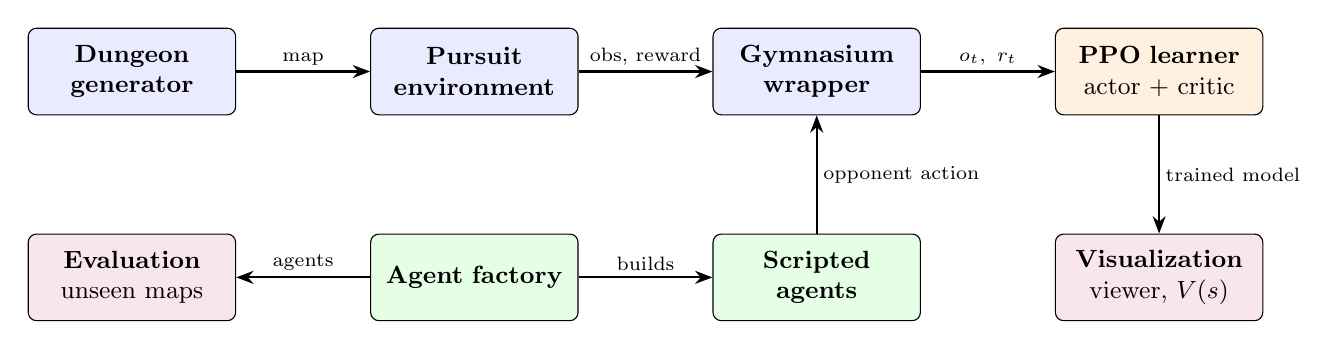
\begin{tikzpicture}[
  box/.style={draw, rounded corners=3pt, align=center, minimum height=1.1cm,
              text width=2.4cm, font=\small, fill=#1},
  box/.default=white,
  arr/.style={-{Stealth[length=2.2mm]}, thick},
  lab/.style={font=\scriptsize, inner sep=2pt}]
\node[box=blue!8] (gen) {\textbf{Dungeon generator}};
\node[box=blue!8, right=1.7cm of gen] (env) {\textbf{Pursuit environment}};
\node[box=blue!8, right=1.7cm of env] (wrap) {\textbf{Gymnasium wrapper}};
\node[box=orange!12, right=1.7cm of wrap] (ppo) {\textbf{PPO learner}\\ actor + critic};
\node[box=purple!10, below=1.5cm of gen] (eval) {\textbf{Evaluation}\\ unseen maps};
\node[box=green!10, below=1.5cm of env] (fac) {\textbf{Agent factory}};
\node[box=green!10, below=1.5cm of wrap] (scr) {\textbf{Scripted agents}};
\node[box=purple!10, below=1.5cm of ppo] (viz) {\textbf{Visualization}\\ viewer, $V(s)$};

\draw[arr] (gen) -- node[lab, above]{map} (env);
\draw[arr] (env) -- node[lab, above]{obs, reward} (wrap);
\draw[arr] (wrap) -- node[lab, above]{$o_t,\ r_t$} (ppo);
\draw[arr] (fac) -- node[lab, above]{builds} (scr);
\draw[arr] (scr) -- node[lab, right]{opponent action} (wrap);
\draw[arr] (fac) -- node[lab, above]{agents} (eval);
\draw[arr] (ppo) -- node[lab, right]{trained model} (viz);
\end{tikzpicture}
\caption{Module architecture at Review II. One role is learned by PPO; the other is played by a
scripted agent inside the wrapper. The agent factory also loads trained PPO models
(\code{ppo:<model>}) for evaluation and the viewer.}
\end{figure}

\begin{center}
\begin{tabularx}{\textwidth}{lX}
\toprule
\textbf{Module} & \textbf{Responsibility}\\
\midrule
\code{env/generator.py} & Rooms, corridors, door, key, obstacles, spawns; validation; seed splits\\
\code{env/dungeon\_env.py} & Rules, simultaneous moves, line-of-sight observations, rewards\\
\code{env/wrappers.py} & \code{SingleAgentEnv}: one role vs a fixed opponent, standard Gymnasium env\\
\code{agents/scripted.py} & Random, Idle, Chase (and oracle) Hunter, Path Evader\\
\code{agents/ppo\_agent.py}, \code{factory.py} & Wrap trained models; build agents from spec strings\\
\code{training/train.py} & PPO training of one role, logging, periodic validation\\
\code{evaluation/} & Matchup table and train / val / test generalization\\
\code{visualization/} & 2.5D renderer, live viewer, HUD, heatmaps, GIF recording, curves\\
\code{tests/test\_env.py} & Generator, rules, capture radius, sprint, Gymnasium API check\\
\bottomrule
\end{tabularx}
\end{center}

%=====================================================================
\section{Design}

\subsection{Game rules}
\begin{itemize}
  \item $21\times21$ grid, 5 rooms, 1 locked door, up to 200 steps. Both agents move at the same
        time with 5 actions: UP, DOWN, LEFT, RIGHT, STAY.
  \item \textbf{Evader wins} by reaching the exit. It needs the key (picked up automatically) to
        open the door that gates the exit.
  \item \textbf{Hunter wins} by catching the Evader: same cell, swapping cells, or within
        \code{capture\_radius}. Otherwise the episode is a timeout.
  \item \textbf{Partial observability}: each agent sees only a $9\times9$ window, and walls, closed
        doors and obstacles block line of sight (Bresenham ray test).
\end{itemize}

\subsection{Balancing the game}
With equal speed and random spawns the Evader won about 99\% of games, so there was nothing for the
Hunter to learn. We added structural Hunter advantages, all configurable:
\begin{center}
\begin{tabular}{lcl}
\toprule
\textbf{Field} & \textbf{Default} & \textbf{Effect}\\
\midrule
\code{hunter\_exit\_dist} & 6 & Hunter spawns within 6 path tiles of the exit (guards it)\\
\code{hunter\_min\_dist} & 8 & Hunter spawns at least 8 tiles from the Evader\\
\code{hunter\_sprint\_every} & 40 & Hunter gets a bonus move every 40th step\\
\code{hunter\_opens\_doors} & true & Hunter walks through doors without a key\\
\bottomrule
\end{tabular}
\end{center}

\subsection{Procedural dungeon generation}
Every map is generated deterministically from an integer seed:
\begin{enumerate}
  \item Place 5 non-overlapping rooms ($3$--$6$ tiles wide) with a wall margin, sort them left to
        right and connect consecutive rooms with L-shaped corridors.
  \item Furnish rooms with obstacle templates (corner crates, L-stack, pillars, colonnade), keeping
        room borders and corridor lanes clear and accepting a tile only if the map stays connected.
  \item Spawn the Evader in a random room and the exit in the room farthest from it.
  \item Place the door on a corridor cell whose closing \emph{disconnects} the exit from the Evader,
        so the door really gates the exit.
  \item Place the key in the region reachable with the door closed, at least 6 tiles from the Evader.
  \item Spawn the Hunter using the balancing constraints above.
  \item \textbf{Validate}: exit and Hunter reachable, key not behind a door, door gates the exit,
        map connected. All 1000 training seeds pass.
\end{enumerate}
\textbf{Seed splits}: train 0--999, validation 10000--10199, test 20000--20499. The splits never
overlap, so evaluation on val/test is always on unseen layouts.

\subsection{Observation, action and reward design}
\begin{itemize}
  \item \textbf{Observation} $o_t\in[-1,1]^{496}$: $9\times9$ window $\times$ 6 binary channels
        (wall, door, key, exit, other agent, visible) $=486$, plus 10 scalars: own position, key
        held, time fraction $t/200$, direction and distance to the current target, other-agent
        visibility and relative position. Hunter target = Evader (when visible); Evader target =
        key while the door blocks the exit, else the exit.
  \item \textbf{Actions}: $\mathcal{A}=\{\text{UP},\text{DOWN},\text{LEFT},\text{RIGHT},\text{STAY}\}$.
  \item \textbf{Reward}: win $+1$ / loss $-1$, step penalty $-0.01$, path-distance shaping $0.01$ per
        tile of progress, Evader $+0.1$ for the key and $+0.1$ for opening the door.
\end{itemize}

%=====================================================================
\section{Connection to Reinforcement Learning}

\subsection{Formulation}
From the learner's viewpoint, with the opponent fixed, the game is a \textbf{partially observable
Markov decision process} (POMDP) $(\mathcal{S},\mathcal{A},P,R,\Omega,O,\gamma)$:
the state $s$ is the full map plus both positions, keys and time; the agent receives the
observation $o=O(s)$ (its $9\times9$ view); the opponent's policy is part of the transition $P$.
With both agents learning, it becomes a two-player \textbf{Markov game}.

\subsection{Value functions, $Q(s,a)$ and sequences of actions}
A \textbf{sequence of actions} produces a trajectory $\tau=(o_0,a_0,r_0,o_1,a_1,r_1,\dots)$ with
return $G_t=\sum_{k\ge0}\gamma^k r_{t+k}$, $\gamma=0.99$. The agent learns
\[
\pi_\theta(a\mid o),\qquad
V^\pi(s)=\E_\pi[G_t\mid s_t=s],\qquad
Q^\pi(s,a)=\E_\pi[G_t\mid s_t=s,a_t=a],\qquad
A^\pi(s,a)=Q^\pi(s,a)-V^\pi(s).
\]
\begin{itemize}
  \item $V(s)$ is learned explicitly by the PPO critic, and we visualize it as a heatmap over the
        map (Section~\ref{sec:viz}).
  \item $Q(s,a)$ is not learned directly; PPO uses the advantage $A(s,a)$, estimated from sequences
        of rewards with GAE (below), to decide which actions to reinforce.
  \item The Bellman equation $V^\pi(s)=\E_{a\sim\pi}[r+\gamma V^\pi(s')]$ gives the TD error used by
        the critic: $\delta_t=r_t+\gamma V(s_{t+1})-V(s_t)$.
\end{itemize}

\subsection{Deep RL algorithm: PPO}
\paragraph{Policy gradient.} $\nabla_\theta J=\E\big[\nabla_\theta\log\pi_\theta(a_t|o_t)\,\hat A_t\big]$:
raise the probability of actions that did better than expected.
\paragraph{GAE.} $\hat A_t=\sum_{l\ge0}(\gamma\lambda)^l\delta_{t+l}$ with $\lambda=0.95$, trading
bias against variance.
\paragraph{Clipped objective.} With ratio $r_t=\pi_\theta(a_t|o_t)/\pi_{\theta_\text{old}}(a_t|o_t)$,
\[
L^{\text{CLIP}}=\E_t\big[\min(r_t\hat A_t,\ \operatorname{clip}(r_t,1-\epsilon,1+\epsilon)\hat A_t)\big],\quad\epsilon=0.2,
\]
\[
\mathcal{L}=-L^{\text{CLIP}}+c_v\,\E_t\big[(V_\theta(o_t)-\hat R_t)^2\big]-c_e\,\E_t\big[\mathcal{H}(\pi_\theta(\cdot|o_t))\big].
\]
Clipping keeps each update close to the previous policy, so the same batch can be reused for
several epochs without collapsing the policy.

\subsection{Network architecture and output}
\begin{figure}[h]
\centering
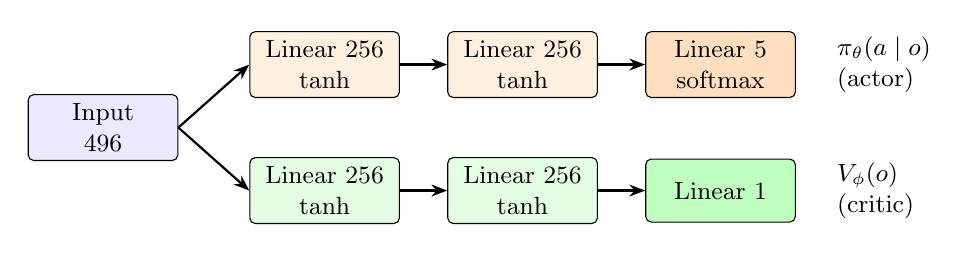
\begin{tikzpicture}[
  lay/.style={draw, rounded corners=2pt, minimum width=1.9cm, minimum height=0.8cm,
              align=center, font=\small, fill=#1},
  lay/.default=white,
  arr/.style={-{Stealth[length=2mm]}, thick}]
\node[lay=blue!8] (in) {Input\\ 496};
\node[lay=orange!12, right=0.9cm of in, yshift=0.8cm] (p1) {Linear 256\\ tanh};
\node[lay=orange!12, right=0.6cm of p1] (p2) {Linear 256\\ tanh};
\node[lay=orange!25, right=0.6cm of p2] (p3) {Linear 5\\ softmax};
\node[right=0.4cm of p3, font=\small, align=left] {$\pi_\theta(a\mid o)$\\ (actor)};
\node[lay=green!10, right=0.9cm of in, yshift=-0.8cm] (v1) {Linear 256\\ tanh};
\node[lay=green!10, right=0.6cm of v1] (v2) {Linear 256\\ tanh};
\node[lay=green!25, right=0.6cm of v2] (v3) {Linear 1};
\node[right=0.4cm of v3, font=\small, align=left] {$V_\phi(o)$\\ (critic)};
\draw[arr] (in.east) -- (p1.west); \draw[arr] (p1) -- (p2); \draw[arr] (p2) -- (p3);
\draw[arr] (in.east) -- (v1.west); \draw[arr] (v1) -- (v2); \draw[arr] (v2) -- (v3);
\end{tikzpicture}
\caption{Actor-critic network: two separate MLPs on the same 496-dim observation.}
\end{figure}
\begin{itemize}
  \item \textbf{Actor output}: 5 logits $\to$ softmax $\to$ a categorical distribution over
        actions. Training samples from it; evaluation took the most probable action.
  \item \textbf{Critic output}: one scalar, the estimated state value $V(o)$.
  \item \textbf{Gradient descent}: the loss $\mathcal{L}$ is minimised with Adam
        (learning rate $3\cdot10^{-4}$) on minibatches of 256 samples, 10 epochs per rollout of
        $8\times256=2048$ steps, with gradient-norm clipping $0.5$.
\end{itemize}
\begin{center}
\begin{tabular}{llll}
\toprule
\textbf{Hyper-parameter} & \textbf{Value} & \textbf{Hyper-parameter} & \textbf{Value}\\
\midrule
Parallel envs & 8 & Discount $\gamma$ & 0.99\\
Rollout length & 256 & GAE $\lambda$ & 0.95\\
Minibatch & 256 & Clip $\epsilon$ & 0.2\\
Epochs & 10 & Entropy coef. & 0.01\\
Learning rate & $3\cdot10^{-4}$ & Hidden layers & 256, 256\\
\bottomrule
\end{tabular}
\end{center}
At Review II, PPO was run through the Stable-Baselines3 implementation. For the final review we
reimplement PPO (and DQN) from scratch.

\subsection{Related Deep RL algorithms and why PPO}
\begin{itemize}
  \item \textbf{DQN} learns $Q(s,a)$ with a replay buffer and target network and acts
        $\arg\max_a Q$. It is off-policy and sample-efficient, but in adversarial training
        old replay data describes an outdated opponent, and its deterministic policy is weak under
        partial observability. We add it as a value-based baseline in the final review.
  \item \textbf{A2C/A3C}: synchronous/asynchronous actor-critic without clipping; PPO is the
        more stable successor that reuses each batch for several epochs.
  \item \textbf{TRPO}: enforces a hard KL trust region with second-order optimisation; PPO
        approximates it with a first-order clipped objective.
  \item \textbf{MCTS} (as in AlphaZero) plans by simulating sequences of actions from the current
        state. It needs the true state and a model of the opponent's moves. Our agents see only a
        partial view and move simultaneously, so tree search does not fit directly; model-free PPO
        learns from experience instead.
\end{itemize}

%=====================================================================
\section{Implementation (Code)}

\subsection{Environment step: simultaneous moves and capture}
\begin{lstlisting}[title={\code{env/dungeon\_env.py} -- excerpt of \code{step}}]
self.t += 1
caught = any(abs(h[0] - e_new[0]) + abs(h[1] - e_new[1]) <= cfg.capture_radius
             for h in h_path) or (h_new == e_old and e_new == h_old)
escaped = e_new == self.exit_pos
term = trunc = False
if caught:
    term, self.outcome = True, "caught"
    rew[HUNTER] += cfg.win_reward
    rew[EVADER] -= cfg.win_reward
elif escaped:
    term, self.outcome = True, "escaped"
    rew[EVADER] += cfg.win_reward
    rew[HUNTER] -= cfg.win_reward
elif self.t >= cfg.max_steps:
    trunc, self.outcome = True, "timeout"
\end{lstlisting}

\subsection{Gymnasium wrapper: one learner vs a fixed opponent}
\begin{lstlisting}[title={\code{env/wrappers.py}}]
class SingleAgentEnv(gym.Env):
    def __init__(self, role, opponent, cfg=None, seeds=None, rng_seed=0):
        super().__init__()
        self.role = role
        self.other = EVADER if role == HUNTER else HUNTER
        self.opponent = opponent
        self.env = DungeonPursuitEnv(cfg or EnvConfig(), seeds=seeds, rng_seed=rng_seed)
        self.observation_space = self.env.observation_space
        self.action_space = self.env.action_space

    def step(self, action):
        opp = self.opponent.act(self.env, self.other)
        obs, rew, term, trunc, info = self.env.step(
            {self.role: int(action), self.other: opp})
        return obs[self.role], float(rew[self.role]), term, trunc, info
\end{lstlisting}

\subsection{Scripted opponents}
\begin{lstlisting}[title={\code{agents/scripted.py} -- Chase Hunter and Path Evader}]
class ChaseHunter(Agent):
    def act(self, env, role=HUNTER):
        me = env.pos[HUNTER]
        if self.oracle or env.sees_other(HUNTER):
            self.target = env.pos[EVADER]          # chase what it sees
        if self.target is None or me == self.target:
            self.target = env.random_floor_tile()  # otherwise patrol
        return env.first_action_toward(me, {self.target}, env.cfg.hunter_opens_doors)


class PathEvader(Agent):
    def act(self, env, role=EVADER):
        me = env.pos[EVADER]
        a = env.first_action_toward(me, env.objective_targets(), env.keys_held > 0)
        if self.flee_radius > 0 and env.sees_other(EVADER):
            h = env.pos[HUNTER]
            if abs(me[0] - h[0]) + abs(me[1] - h[1]) <= self.flee_radius:
                def score(k):
                    p, _ = env.resolve_move(EVADER, k)
                    return (abs(p[0] - h[0]) + abs(p[1] - h[1]), k == a)
                a = max(range(5), key=score)        # step away from the Hunter
        return a
\end{lstlisting}

\subsection{PPO training setup}
\begin{lstlisting}[title={\code{training/train.py} -- model construction and training}]
fns = [make_env(role, opp, train_seeds, cfg, args.seed * 1000 + i)
       for i in range(args.n_envs)]
venv = SubprocVecEnv(fns) if args.subproc else DummyVecEnv(fns)

model = PPO("MlpPolicy", venv, n_steps=256, batch_size=256, n_epochs=10,
            learning_rate=3e-4, gamma=0.99, gae_lambda=0.95, ent_coef=args.ent_coef,
            policy_kwargs=dict(net_arch=[256, 256]), device="cpu", verbose=0)

cb = LogCallback(role, opp, cfg, val_seeds, args.eval_freq, out)
model.learn(total_timesteps=args.steps, callback=cb)
\end{lstlisting}

\subsection{Explainability: value heatmap $V(s)$}
\label{sec:viz}
We place the agent on every walkable cell, build its observation and query the critic. The result
shows where the agent believes it is winning.
\begin{lstlisting}[title={\code{visualization/live.py} -- value\_heatmap}]
def value_heatmap(agent, env, role):
    model = agent.model
    heat = np.full((env.H, env.W), np.nan)
    saved = env.pos[role]
    for r in range(env.H):
        for c in range(env.W):
            if env.grid[r, c] == WALL:
                continue
            env.pos[role] = (r, c)
            obs_t, _ = model.policy.obs_to_tensor(env.observe(role))
            with torch.no_grad():
                heat[r, c] = float(model.policy.predict_values(obs_t)[0, 0])
    env.pos[role] = saved
    lo, hi = np.nanmin(heat), np.nanmax(heat)
    return (heat - lo) / (hi - lo + 1e-9)
\end{lstlisting}
The live viewer also draws the actor's action probabilities $\pi(a|o)$ as arrows around each PPO
agent, with toggles for vision cones, trails and the heatmap.

%=====================================================================
\section{Results}

\subsection{Scripted and PPO matchups (validation maps, 100 unseen maps)}
\begin{center}
\begin{tabular}{llcccc}
\toprule
\textbf{Hunter} & \textbf{Evader} & \textbf{H win} & \textbf{E win} & \textbf{Timeout} & \textbf{Mean len}\\
\midrule
random & random & 0.03 & 0.00 & 0.97 & 196.9\\
chase & random & 0.99 & 0.00 & 0.01 & 43.0\\
random & path & 0.06 & 0.93 & 0.01 & 50.6\\
chase & path & 0.39 & 0.61 & 0.00 & 44.0\\
chase\_oracle & path & 0.49 & 0.51 & 0.00 & 43.5\\
\midrule
PPO hunter (vs path) & path & \textbf{0.43} & 0.21 & 0.36 & 114.1\\
PPO hunter (vs path) & random & 0.00 & 0.00 & 1.00 & 200.0\\
PPO hunter (vs random) & path & 0.17 & 0.78 & 0.05 & 53.3\\
PPO hunter (vs random) & random & 0.09 & 0.00 & 0.91 & 191.2\\
chase & PPO evader (vs chase) & 0.49 & \textbf{0.42} & 0.09 & 74.5\\
random & PPO evader (vs chase) & 0.01 & 0.11 & 0.88 & 185.1\\
\bottomrule
\end{tabular}
\end{center}

\subsection{Generalization (train maps vs unseen maps)}
\begin{center}
\begin{tabular}{lcccc}
\toprule
\textbf{Agent} & \textbf{Budget} & \textbf{Train maps} & \textbf{Val maps} & \textbf{Test maps}\\
\midrule
PPO Hunter vs path & 300k steps, 10.5 min & 0.30 & 0.42 & 0.40\\
PPO Evader vs chase & 600k steps, 16.9 min & 0.38 & 0.48 & --\\
PPO Hunter vs random & 300k steps, 10.7 min & 0.00 & 0.00 & --\\
\bottomrule
\end{tabular}
\end{center}

\subsection{Observations}
\begin{itemize}
  \item \textbf{The game is balanced.} The scripted chase vs path matchup is 0.39 / 0.61, and an
        oracle Hunter that always knows where the Evader is gets 0.49. Before balancing, the Evader
        won about 99\%.
  \item \textbf{PPO Hunter $\approx$ best scripted Hunter.} Trained against the path Evader, PPO
        reaches 0.43 on unseen maps, above chase (0.39) and close to the oracle (0.49), without
        cheating information.
  \item \textbf{No overfitting to layouts.} Win rates on unseen val/test maps (0.40--0.48) are
        not lower than on training maps (0.30--0.38): the agents learn general behaviour, not
        memorised maps.
  \item \textbf{Overfitting to the opponent.} The PPO Hunter trained against path only walks toward
        an Evader it can see, so it never catches a random Evader (timeout 1.00). Agents generalize
        across maps, but not across opponents. This motivates self-play in the final review.
  \item \textbf{Sparse reward.} The Hunter trained against a random Evader barely learns: random
        movement gives almost no catches to learn from. This motivates curriculum learning.
\end{itemize}

%=====================================================================
\section{Innovation, with Proof}
\begin{center}
\begin{tabularx}{\textwidth}{p{4.2cm}X}
\toprule
\textbf{Innovation} & \textbf{Proof / evidence}\\
\midrule
Generalization is measured, not assumed: disjoint procedural seed splits (train/val/test) &
Every result above is on unseen maps; PPO Hunter 0.30 train vs 0.40 test shows no layout
overfitting.\\
Solvable-by-construction generator with a door on a \emph{cut} corridor &
The door is placed only where closing it disconnects the exit from the Evader; the validator checks
all 1000 training seeds (\code{python -m env.generator}).\\
Asymmetric balancing of an adversarial game &
Evader won $\sim$99\% with equal rules; after adding guard spawn and sprint the scripted matchup is
0.39 / 0.61 and the oracle 0.49 / 0.51.\\
Partial observability with line of sight in a pursuit game &
$9\times9$ Bresenham line-of-sight window; the oracle Hunter (full information) beats the
normal chase Hunter by 0.10, which quantifies the value of information.\\
Interpretable agents: live $V(s)$ heatmap and action-probability arrows &
Implemented in the live viewer (\code{H} and arrow overlays); shows where the critic predicts a
win and what the actor intends.\\
Opponent-overfitting finding that drives the next phase &
PPO Hunter vs path: 0.43 vs path but 0.00 vs random; evidence that single-opponent training is
brittle and motivates self-play and exploitability tests.\\
\bottomrule
\end{tabularx}
\end{center}

%=====================================================================
\section{Contribution of Team Members}
\begin{center}
\begin{tabularx}{\textwidth}{lX}
\toprule
\textbf{Member} & \textbf{Contribution}\\
\midrule
Aayush Shukla (23BPS1081) &
Procedural dungeon generator and validation; environment rules, line-of-sight observations and
reward design; game balancing (guard spawn, sprint); PPO training script and logging;
generalization evaluation on seed splits.\\
Aditya Kumar (23BPS1163) &
Scripted agents (chase, oracle, path, random) and agent factory; Gymnasium wrapper and tests;
matchup evaluation and baseline table; 2.5D renderer, live viewer, HUD, value heatmap and
action-probability overlays; GIF recording and training-curve plots.\\
Both &
Problem formulation, experiment design, analysis of results and this report.\\
\bottomrule
\end{tabularx}
\end{center}

%=====================================================================
\section{Plan for the Final Review}
\begin{itemize}
  \item Implement PPO and DQN from scratch (no RL libraries) and a faster multi-process environment.
  \item Simultaneous adversarial training: independent learners vs self-play with a frozen-opponent pool.
  \item Adaptive curriculum over map size, doors, obstacles and opponent skill.
  \item Exploitability test: freeze a trained agent and measure how fast a fresh agent beats it.
  \item Out-of-distribution maps ($25\times25$, two doors), cross-play stability matrices, decision
        heatmaps and a results dashboard.
\end{itemize}

\section*{References}
\begin{enumerate}[label={[\arabic*]},leftmargin=*]
  \item J. Schulman et al. \emph{Proximal Policy Optimization Algorithms.} arXiv:1707.06347, 2017.
  \item J. Schulman et al. \emph{High-Dimensional Continuous Control Using Generalized Advantage Estimation.} ICLR, 2016.
  \item V. Mnih et al. \emph{Human-level control through deep reinforcement learning.} Nature, 2015.
  \item D. Silver et al. \emph{Mastering the game of Go without human knowledge.} Nature, 2017.
  \item K. Cobbe et al. \emph{Leveraging Procedural Generation to Benchmark Reinforcement Learning.} 2019.
  \item A. Raffin et al. \emph{Stable-Baselines3: Reliable Reinforcement Learning Implementations.} JMLR, 2021.
  \item R. Sutton, A. Barto. \emph{Reinforcement Learning: An Introduction.} 2nd ed., 2018.
\end{enumerate}

\end{document}
